\section{Metodologia de Avaliação e Desempenho Individual} \label{sec:desempenho_individual}

A atribuição de responsabilidades no decorrer deste projeto ocorreu de forma orgânica. Após uma fase inicial de investigação e exploração das tecnologias adotadas, a divisão de tarefas consolidou-se naturalmente: o desenvolvimento da aplicação cliente (\textit{front-end}), que ficou a cargo do Hugo, e a arquitetura e desenvolvimento do servidor (\textit{back-end}), assumida pelo Diogo. 

\subsection{Critérios de Atribuição de \textit{Story Points}}
A atribuição de \textit{Story Points} foi realizada com base na escala de Fibonacci. Esta métrica avaliou a complexidade técnica, o número de operações envolvidas e as integrações necessárias de cada tarefa de desenvolvimento:
\begin{itemize}
	\item \textbf{1 a 3 pontos (Complexidade Baixa a Média-Baixa):} Tarefas com requisitos bem definidos, configurações base (como a injeção de dependências ou estrutura inicial da aplicação), definição da API GraphQL ou parametrizações simples na interface gráfica (como definir limites para os gráficos radiais).
	\item \textbf{5 pontos (Complexidade Média):} Tarefas com integrações entre múltiplos componentes do sistema, construção do \textit{Dashboard} interativo ou configuração das pontes MQTT e GraphQL \textit{Subscriptions}.
	\item \textbf{8 pontos (Complexidade Alta):} Tarefas tecnicamente desafiantes, exigindo manipulação assíncrona de eventos, orquestração contínua do simulador de dados e renderização de séries temporais reativas combinadas com histórico.
\end{itemize}

\subsection{Distribuição do Esforço e Contribuição}
Após a atribuição e somatório dos \textit{Story Points} (SP) de todas as fases do projeto, apurou-se um total de 68 SP. A Figura \ref{fig:distribuicao_sp} ilustra a distribuição global do esforço:

\begin{figure}[h]
	\centering
	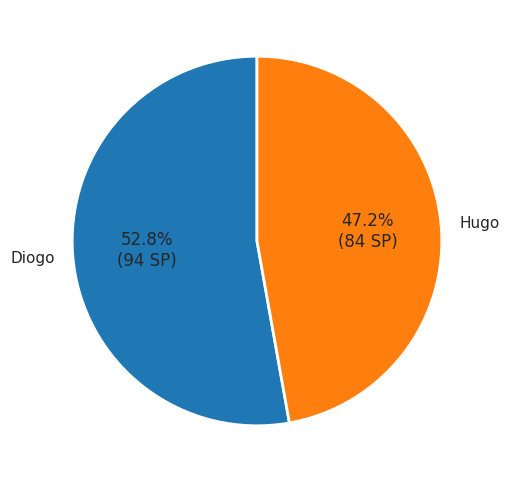
\includegraphics[width=0.5\textwidth]{imagens/desempenho_individual_story_points.png} 
	\caption{Distribuição da carga de trabalho do projeto com base em \textit{Story Points}.}
	\label{fig:distribuicao_sp}
\end{figure}

\subsubsection{Contribuição: Diogo (52.8\% -- 94 SP)}
O Diogo assumiu a responsabilidade pela arquitetura e desenvolvimento do \textit{back-end} em \textit{Scala} utilizando o ecossistema \textit{ZIO}. A sua carga de trabalho esteve concentrada no processamento não-bloqueante de dados e na infraestrutura reativa:
\begin{itemize}
	\item \textbf{Simulador e Integração MQTT:} A tarefa mais exigente do \textit{back-end} (avaliada em 8 SP), que envolveu a integração e orquestração do simulador de sensores IoT, garantindo o correto fluxo de dados em formato \textit{Sparkplug B} através do \textit{broker} MQTT.
	\item \textbf{Processamento de Eventos:} Tarefas de média-alta complexidade relativas ao processamento em memória do estado dos nós (\textit{Nodes}) e telemetrias (\textit{Metrics}), recorrendo à programação orientada a eventos.
	\item \textbf{Motor GraphQL e Base de Dados:} Configuração da infraestrutura persistente (\textit{PostgreSQL}) e implementação da API GraphQL (com recurso à biblioteca \textit{Caliban}), culminando na gestão das \textit{subscriptions} reativas.
\end{itemize}

\subsubsection{Contribuição: Hugo (47.2\% -- 84 SP)}
O Hugo assumiu a estruturação, lógica e interface visual do cliente interativo (\textit{front-end}) em \textit{Flutter}. A sua contribuição focou-se no domínio de apresentação reativa, sincronização de estado (\textit{MVVM}) e componentes visuais de análise:
\begin{itemize}
	\item \textbf{Gráficos e Séries Temporais:} A tarefa de maior exigência técnica no cliente, que consistiu em fundir dados históricos com eventos em tempo real provenientes das \textit{subscriptions}, traduzindo-os em gráficos de linhas dinâmicos (\textit{Time Series Charts}).
	\item \textbf{Sincronismo em Tempo Real:} Configuração complexa do cliente GraphQL no lado da aplicação móvel/web, gerindo as sessões \textit{WebSocket} para a atualização contínua de dados.
	\item \textbf{Dashboard Visual:} O desenvolvimento do ecrã de controlo, que incluiu a renderização dos mostradores radiais (\textit{Gauges}), permitindo ainda configurações locais personalizadas de limites mínimos e máximos.
\end{itemize}